
%Volume: maximaal aantal pagina van inleiding t/m literatuur, maximaal  35 bladzijden (excl.bijlagen).
\documentclass[11pt]{report}
\usepackage[a4 paper, headheight=1pt, headsep=1pt] {geometry}
\usepackage{titlesec}
\titleformat{\chapter}[display]   
{\normalfont\huge\bfseries}{\chaptertitlename\ \thechapter}{8pt}{\huge}   
\titlespacing*{\chapter}{0pt}{-65pt}{8pt}
\titlespacing*{\section}{0pt}{5pt}{1pt}
\setlength{\parindent}{0pt}
\setlength{\parskip}{5pt plus 2pt minus 1pt}
\setlength{\textheight}{680pt}
\setlength{\headsep}{0pt}
%\usepackage{showframe}
\usepackage{graphicx}
\usepackage[usenames,dvipsnames]{color}
%\usepackage{picins}
\footskip = 20pt 
\usepackage[nodayofweek]{datetime}
\usepackage{tikz}
\usepackage{todonotes}
\usetikzlibrary{shapes.geometric, arrows}
\usepackage{pdfpages}
\usepackage{xcolor}

\begin{document}
\begin{titlepage}
	\begin{center}
	\vspace*{0\textheight}
	{\scshape\LARGE Utrecht University \par}
	\vspace{1cm} 
	\line(4,0){300}
	\vspace{0.5cm} \\
	{\Large \bfseries Still unknown}
	\vspace{0.5cm}
	\line(4,0){300} \\

	\vspace{2.5cm}
	\begin{minipage}[t]{0.4\textwidth}
	\begin{flushleft} \large
	\emph{Author:}\\
	{Isolde Glissenaar}\\
	{Daphne van Zanten} \\
	\end{flushleft}
	\end{minipage} %No ENTER BECAUSE!
	\begin{minipage}[t]{0.4\textwidth}
	\begin{flushright} \large
	\emph{Supervisor:} \\
	{Dr. C.H. Tijm-Reijmer}\\
	\end{flushright}
	\end{minipage}\\[0.4cm]

	\vspace{3.5cm}
	\large \textit{}\\[1cm]

	{\large {\today}\\[2cm] % Date

	\noindent
	
\includegraphics[scale=1, width=0.35\textwidth]{UU-logo.jpg}}
	\end{center}
\end{titlepage}

\newpage
\tableofcontents

\chapter{Introduction}\label{sec:intro}
\pagenumbering{arabic}
\setcounter{page}{2}
\todo{In report: \\
- General description experiment and conditions\\
– General description of the dataset and data handling\\
– Detailed analyses of chosen subject\\
+- 15 pages}

\newpage

\chapter{Method}\label{sec:method}
\textcolor{red}{location of measurements, instruments, data handling (on making the daily averages and handling the data gaps.)}

\section{Location}
This study discusses data from weather stations situated on Svalbard, which is a Norwegian archipelago in the Arctic Ocean, north of the European mainland. The island group ranges from 74$^\circ$N to 81$^\circ$N in latitude. The archipelago features an Arctic climate, although with higher temperatures than other areas on the same latitude. \textcolor{red}{MEAN TEMP}. The northernmost branch of the relatively warm North Atlantic Current, the West Spitsbergen Current, moderates the temperature on the western side of the island. The East Spitsbergen Current brings colder water from higher latitudes to the eastern side of the archipelago. All three measurement locations are situated on the largest island, called Spitsbergen. 

Data are used from two weather stations from the Institute for Marine and Atmospheric research Utrecht (IMAU) located on two glaciers and data from an operational station from the Norwegian Meteorological Institute. 

The weather stations are situated on the Nordenskiöldbreen and the Ulvebreen. The Nordenskiöldbreen is a marine-terminating glacier, terminating in Adolfsbukta, which is a branch of Billefjorden. The glacier is situated roughly in the middle of the island Spitsbergen. 

\includegraphics[scale=1, width=0.35\textwidth]{currents_svalbard.jpg}
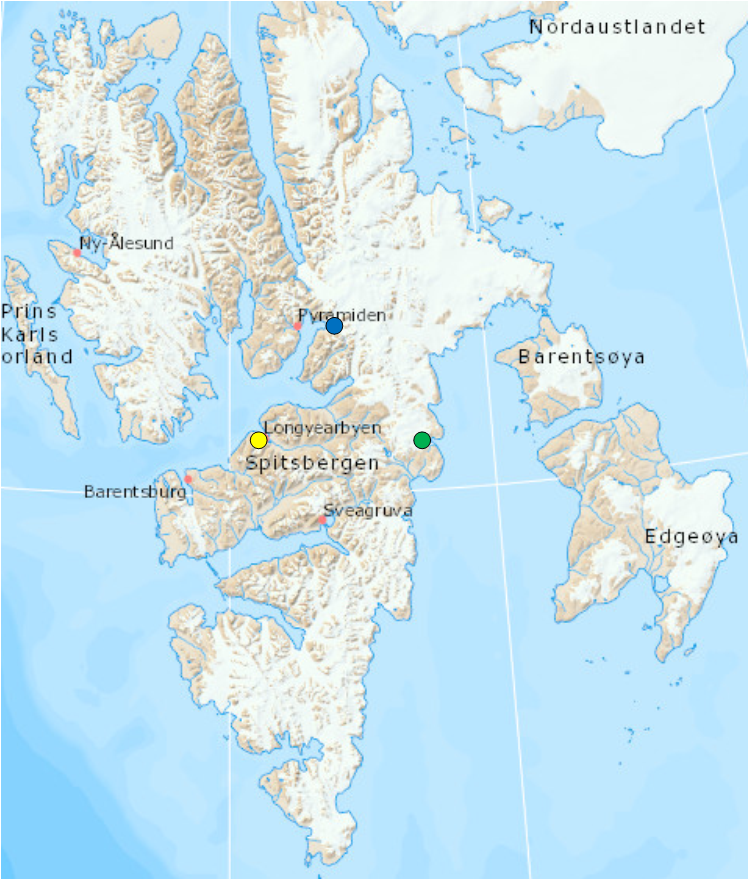
\includegraphics[scale=1, width=0.35\textwidth]{svalbard_locations.png}


%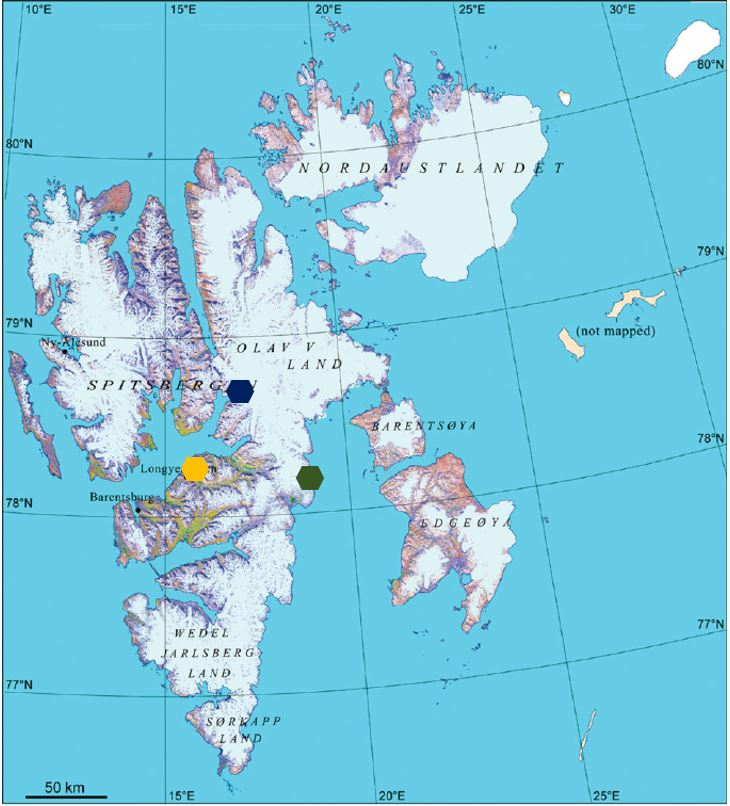
\includegraphics[scale=1, width=0.35\textwidth]{map.jpg}

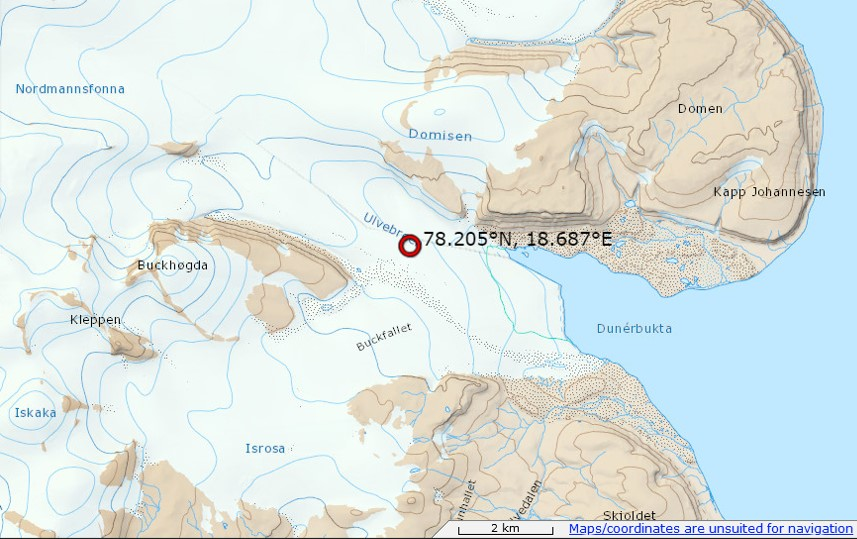
\includegraphics[scale=1, width=0.35\textwidth]{ulvemap.jpg}
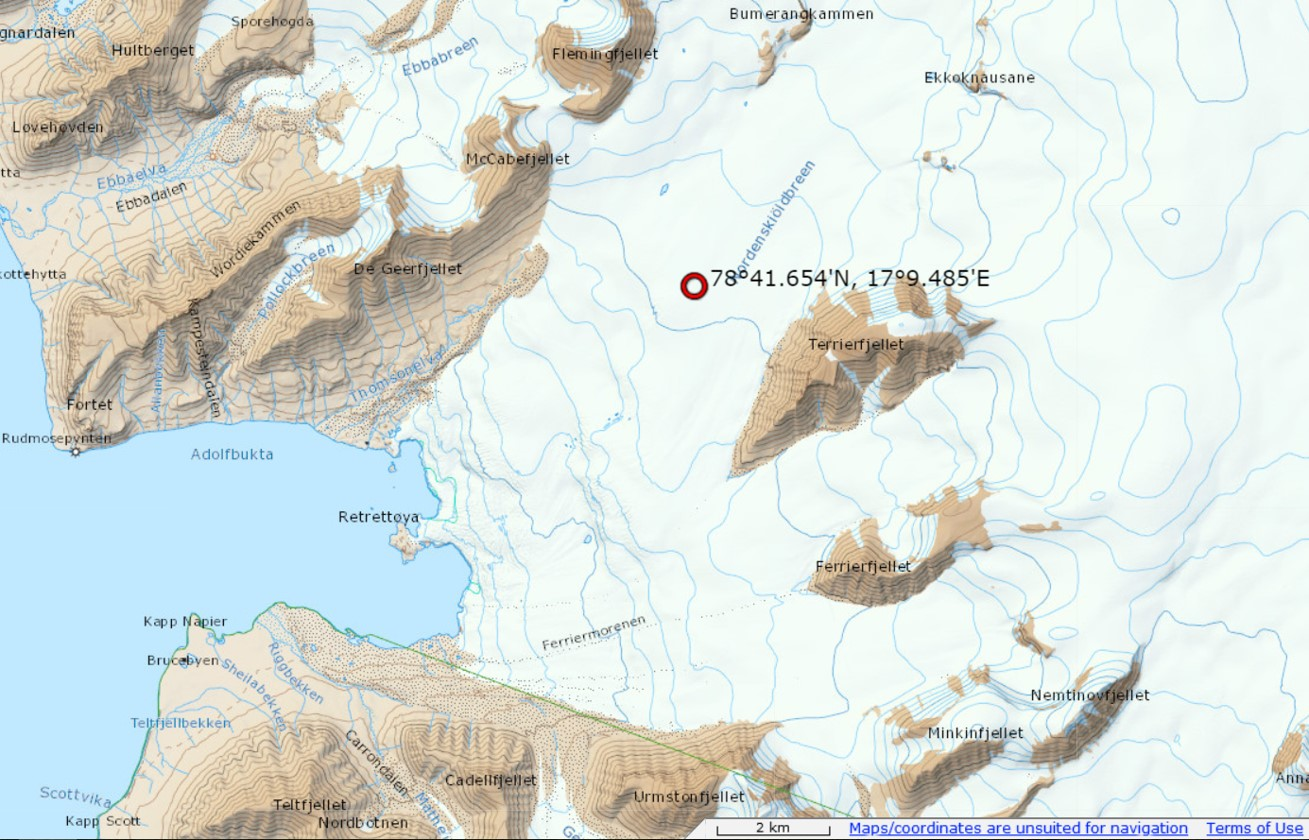
\includegraphics[scale=1, width=0.35\textwidth]{nskimap.jpg}

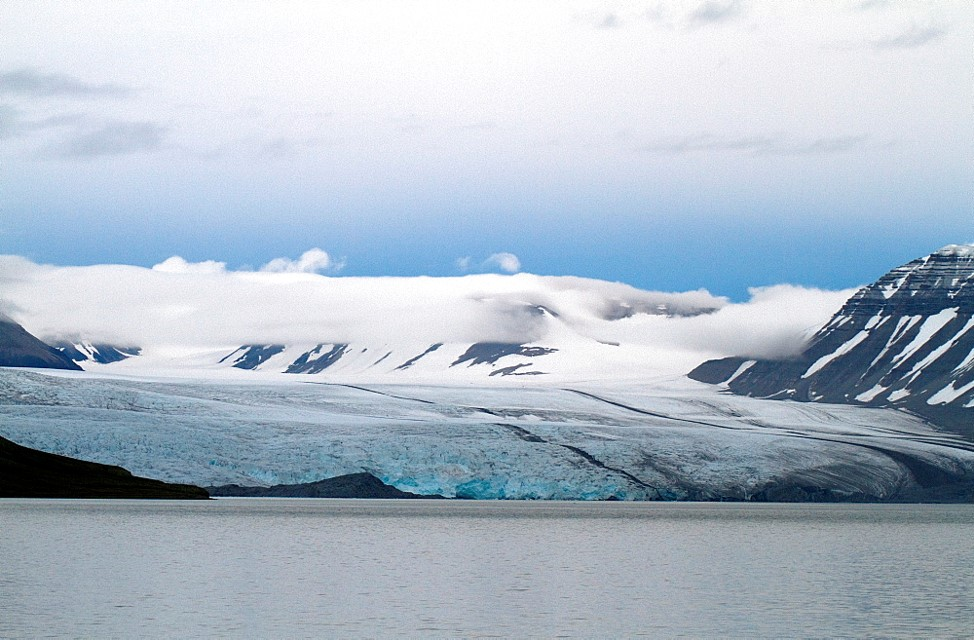
\includegraphics[scale=1, width=0.35\textwidth]{view1.jpg}
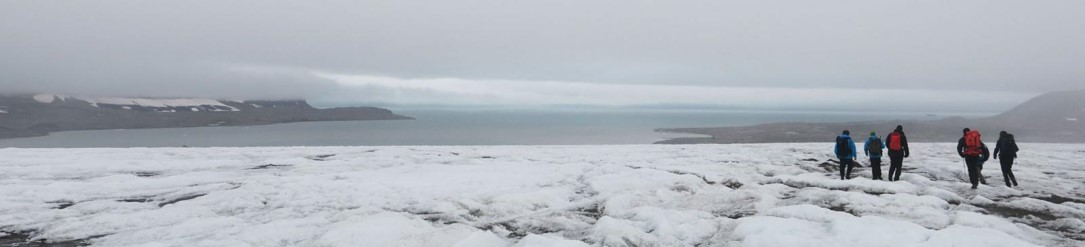
\includegraphics[scale=1, width=0.35\textwidth]{view2.jpg}

\newpage
\section{Instruments}
Instruments used are automatic weather stations, as visible in figures \ref{fig:instrumentn} and \ref{fig:instrumentu}. Both stations are placed as part of the Netherlands Scientific Expedition Edgeøya Spitsbergen in 2015.

Equipment on the Nordenskioldbreen are measuring each 30 minutes different variables. For example the the horizontal wind speed wind direction, 
a radiometer with two pyranometers which is measure the shortwave and longwave incoming and outgoing radiation.
Also the netto temperature of the radiometer is measured.
The surface temperature is derived from the outgoing longwave radiation.
A barometer is measuring the pressure. 
The sonic snow height is measured with a quality number. 
The Potential temperature is based on the main hut temperature and pressure. 
The temperature at 2 meter is based on the main hut temperature and the sonic snow height. 
The specific humidity is based on the main hut temperature and pressure as well. 
Theoretically, the snow temperature is measured at 10 different locations on thing.
A cinclometer is used to measure the tilt. 
Finally, the battery is logged as well as the temperature in the logger, to look at the status of the equipment itself. 

For the ulvebreen, also each 30 minutes a measurement is saved. Measurements of the Ulvebreen are slightly different in some ways compared to the Nordenskioldbreen. 
Instead of snow height at 10 different locations, it are 8 different locations. 
In addition to the Nordenskioldbreen, a abliation draw wire is added to measure 

Two thermocouples are measuring the temperature.

The relative humidity is corrected for air temperature

Heading of magnetic compass, GPS height above mean sea leel, latitude, longitude


And finally again this time the lithium battery usage time and power supply voltage. 
 
ADW[m]			= ABLATION DRAW WIRE
HMSL[m]		= GPS HEIGHT ABOVE MEAN SEA LEVEL 

\begin{figure}[h]
\raggedright
\begin{minipage}{0.5\textwidth}
\raggedright
    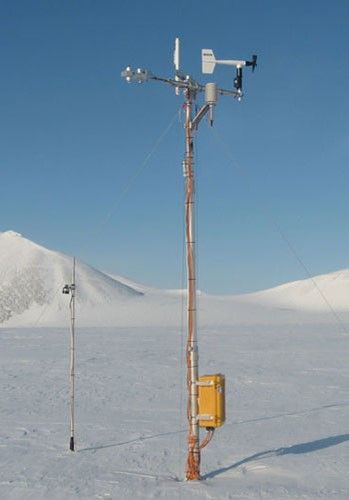
\includegraphics[width=0.7\textwidth]{nski.jpg}
    \label{fig:instrumentn}
    \caption{AWS Nordenskioldbreen - Helga van Leur}
\end{minipage}%
\begin{minipage}{0.5\textwidth}
\raggedright
    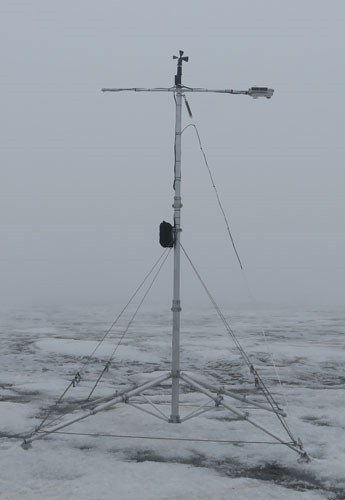
\includegraphics[width=0.7\textwidth]{ulve.jpg}
    \label{fig:instrumentu}
    \caption{AWS Ulvebreen - Helga van Leur}
\end{minipage}%
\end{figure}

\section{Data handling}



\newpage
\chapter{Results}\label{sec:results}

\begin{figure}[h]
\raggedright
\begin{minipage}{0.65\textwidth}
\raggedright
    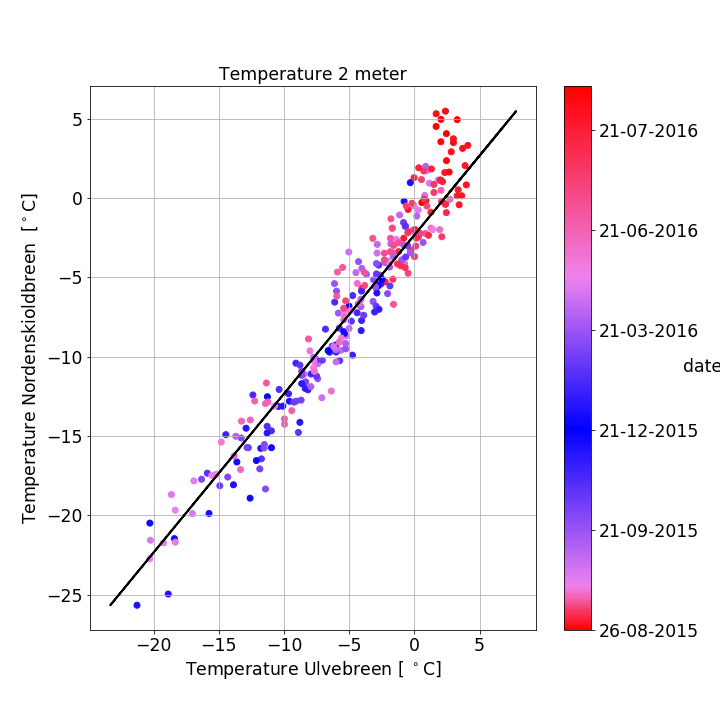
\includegraphics[scale=1, width=1\textwidth]{T2mUlve-T2mNorde.png}	 
    \label{fig:labe}
    \caption{Title}
\end{minipage}%
\end{figure}


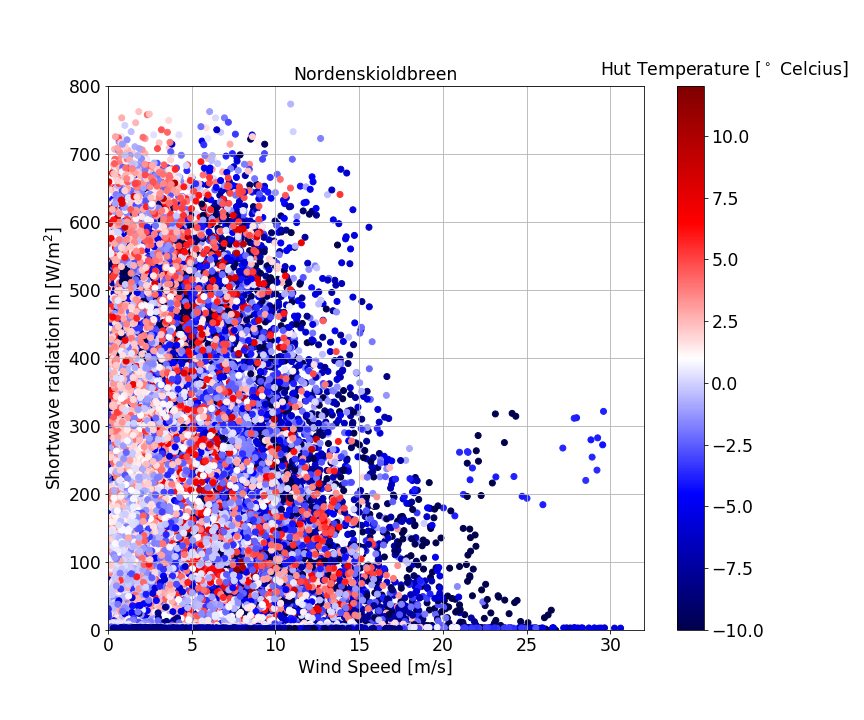
\includegraphics[scale=1, width=0.35\textwidth]{THUT-SIN-WS-Nordenskioldbreen.png}
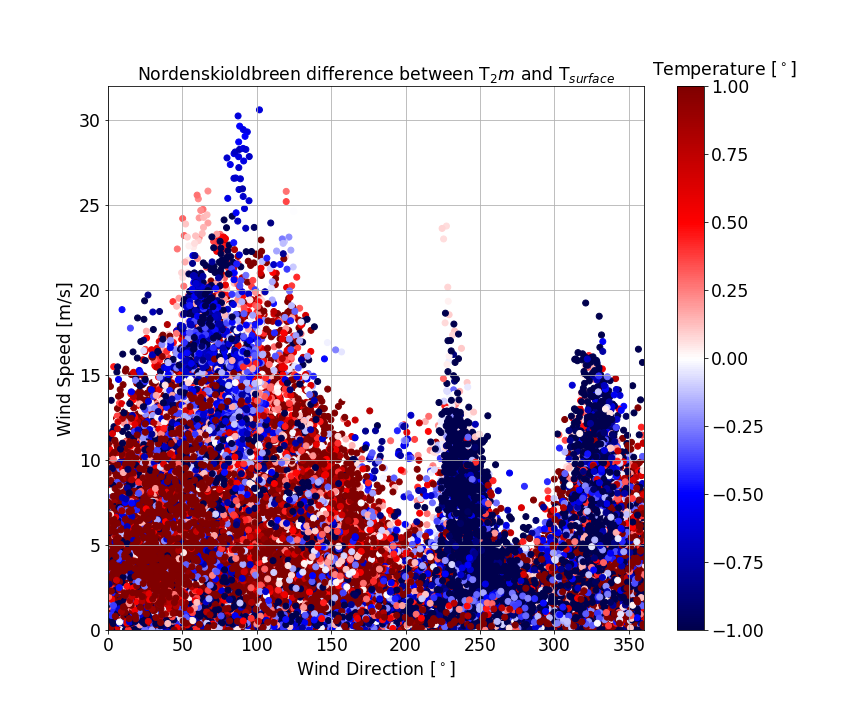
\includegraphics[scale=1, width=0.35\textwidth]{THUT-T2m-WD-WS-Nordenskioldbreen.png}
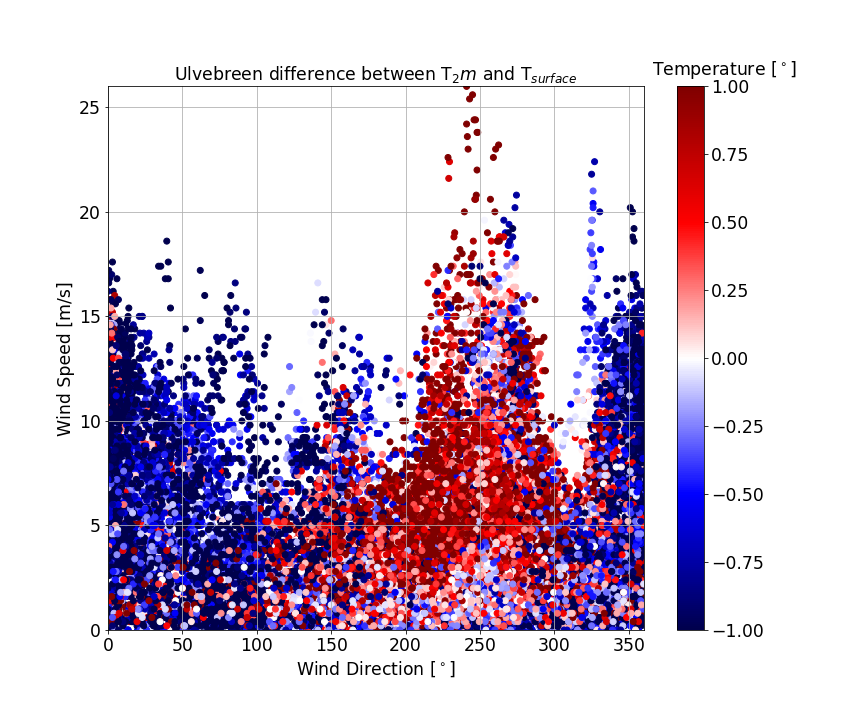
\includegraphics[scale=1, width=0.35\textwidth]{THUT-T2m-WD-WS-Ulvebreen.png}

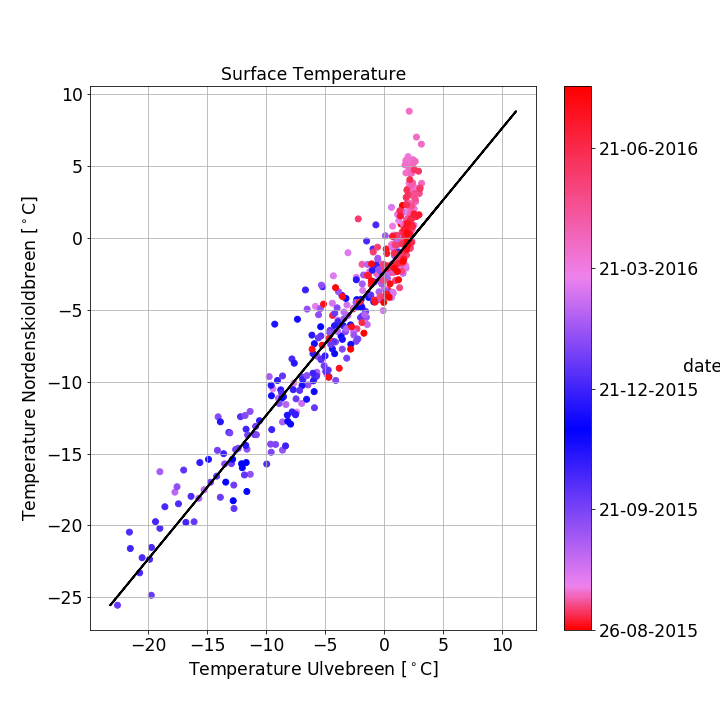
\includegraphics[scale=1, width=0.35\textwidth]{TsurfU-N.png}
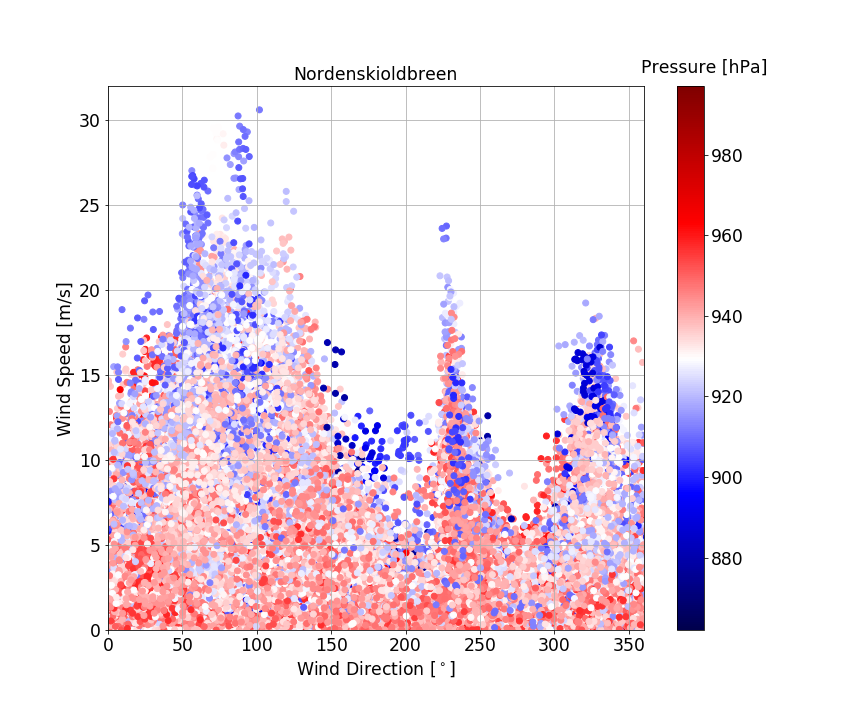
\includegraphics[scale=1, width=0.35\textwidth]{WD-WS-PR-Nordenskioldbreen.png}
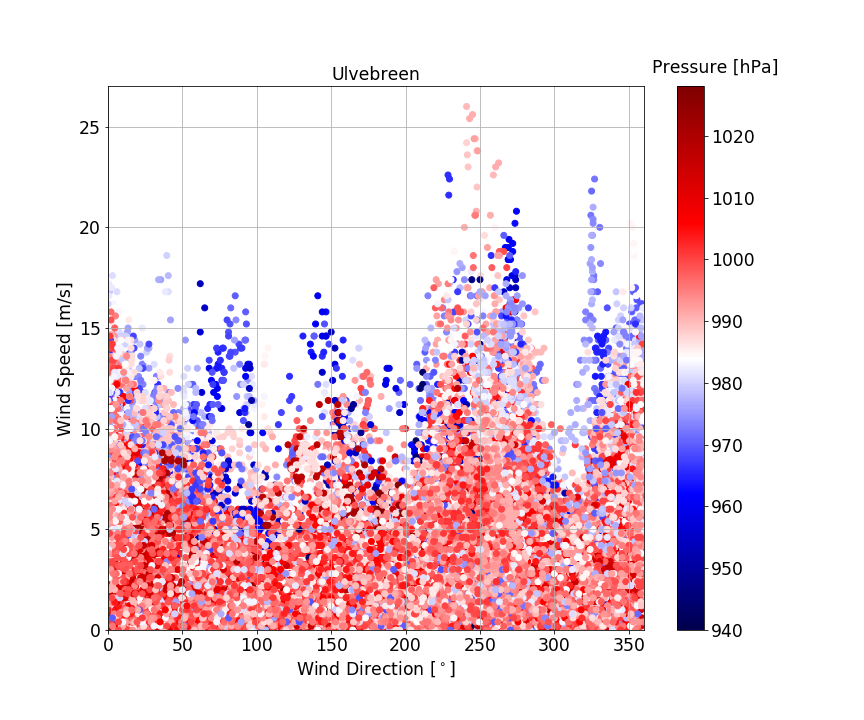
\includegraphics[scale=1, width=0.35\textwidth]{WD-WS-PR-Ulvebreen.png}
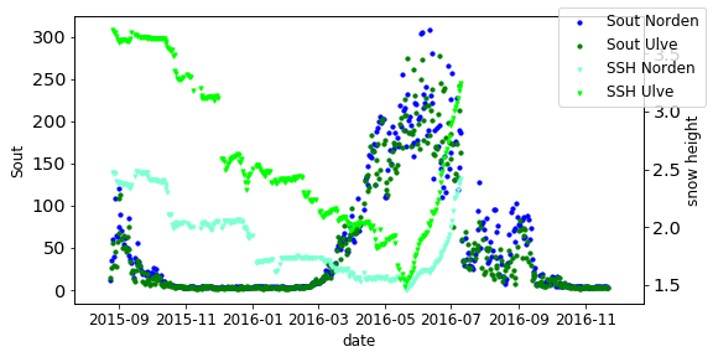
\includegraphics[scale=1, width=0.35\textwidth]{Picture1.jpg}
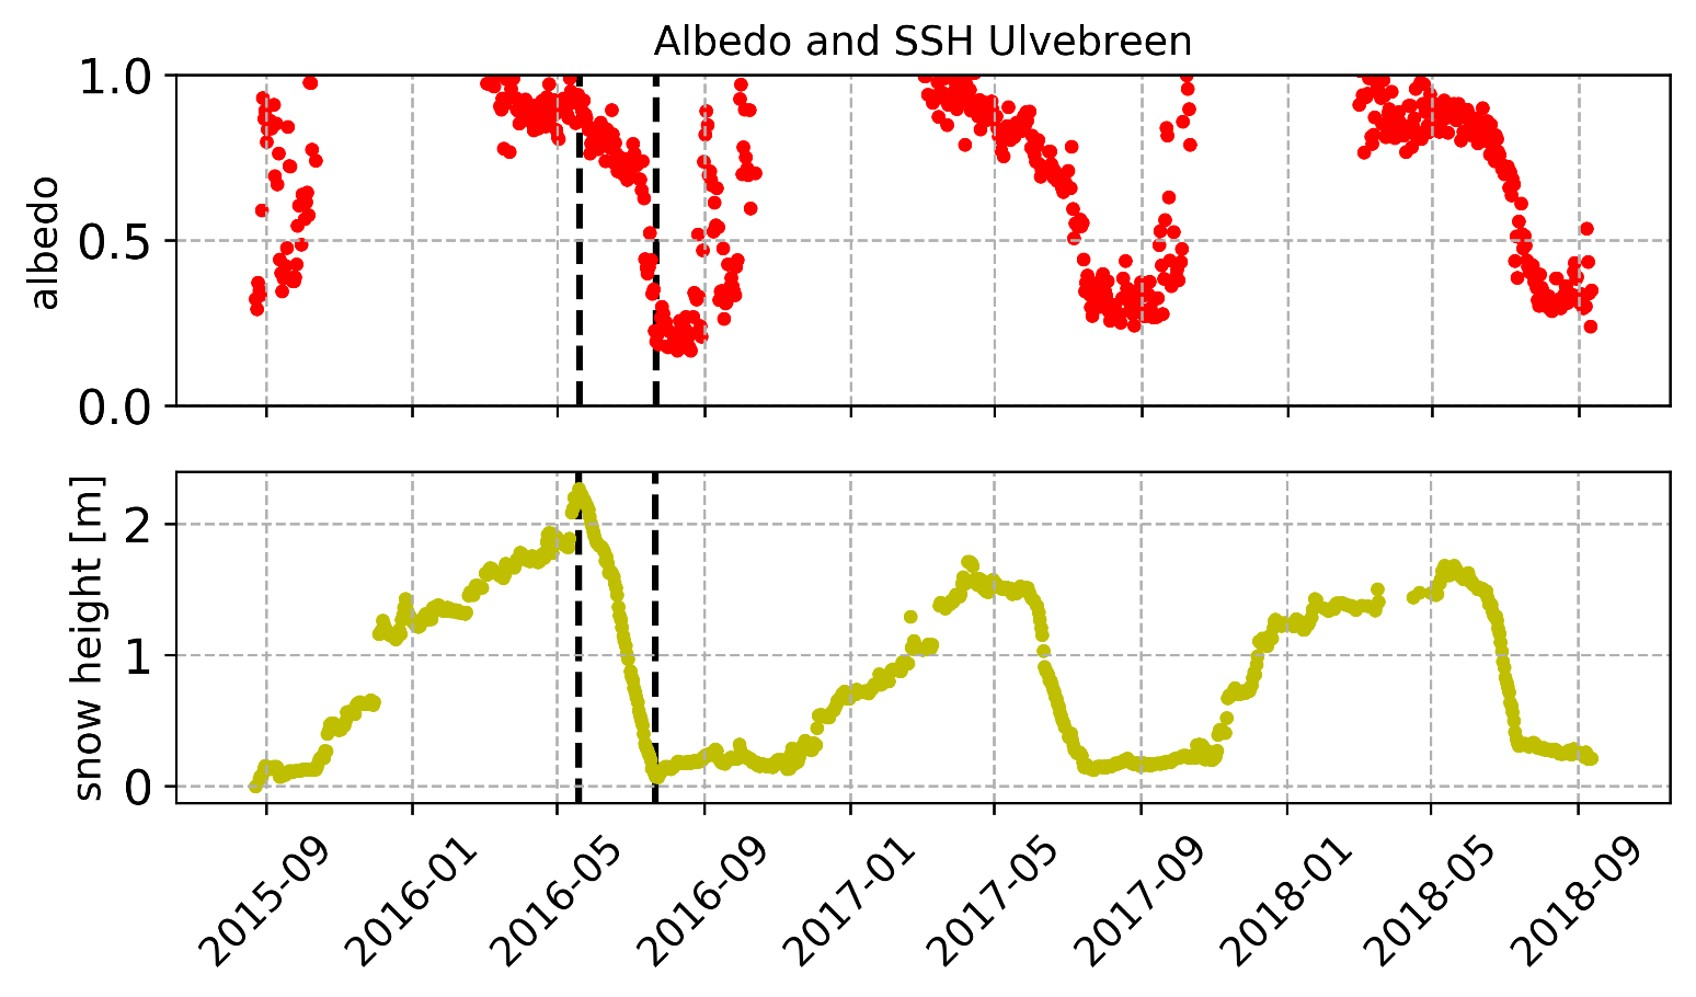
\includegraphics[scale=1, width=0.35\textwidth]{Picture2.jpg}


\chapter{Discussion}\label{sec:discussion}
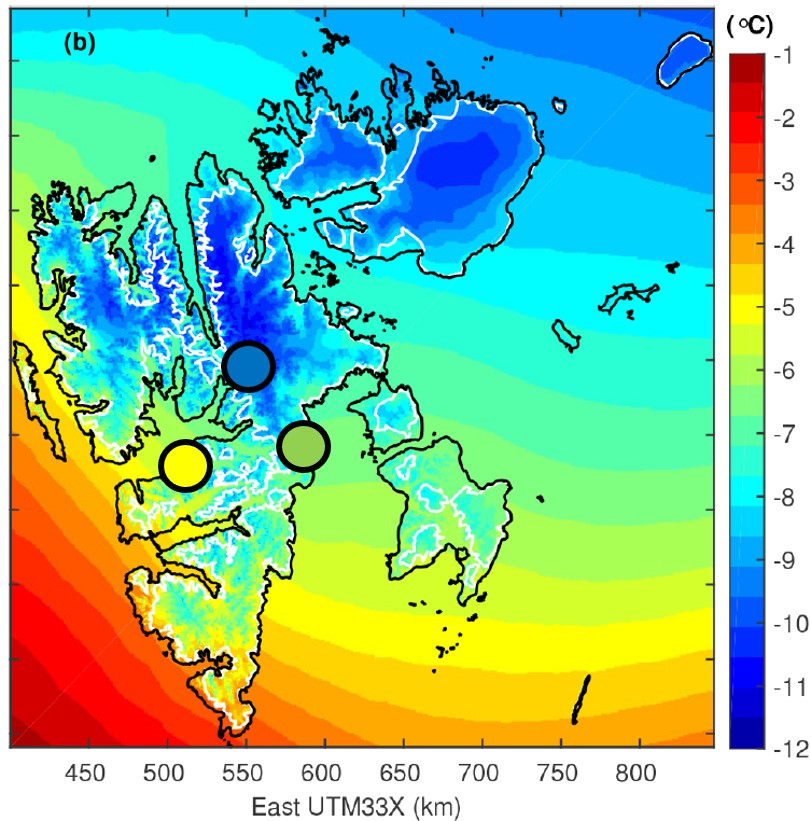
\includegraphics[scale=1, width=0.35\textwidth]{ostby.jpg}
\chapter{Conclusion}\label{sec:conclusion}


\medskip

\begin{thebibliography}{9}
\addcontentsline{toc}{chapter}{Bibliography}
%1
\bibitem{fdj}
Article: de Jong, M. F. et al. (2018) 
\textit{The subsurface circulation of the Iceland Sea observed with RAFOS floats}

\end{thebibliography}

\chapter*{Appendices}
\addcontentsline{toc}{chapter}{Appendices}

\section*{A. name}\label{Ap:A}
\setcounter{figure}{0}
\renewcommand{\thefigure}{A.\arabic{figure}}
\addcontentsline{toc}{section}{A. name}

\end{document}
